%%%%%%%%%%%%%%%%%%%%%%%%%%%%%%%%%%%%%%%%%%%%%%%%%%%%%%%%%%%%%%%%%%%%%%%%%%%%%%%%%%%%%%%%%%%%%%%%%%%%%%%%%
%Atualizado para o CONICT 2026 - Guarulhos pelo professor João Alves Pacheco
%Data: 06/07/2026
%%%%%%%%%%%%%%%%%%%%%%%%%%%%%%%%%%%%%%%%%%%%%%%%%%%%%%%%%%%%%%%%%%%%%%%%%%%%%%%%%%%%%%%%%%%%%%%%%%%%%%%%%

\documentclass[a4paper,11pt]{article}

%PACOTES ABNT
\usepackage[brazil]{babel} % Pacote para usar portugues.
%Babel traduz como “table of contents“, “chapter” e “section“, sejam impressas como “sumário”, “capítulo” e “seção”, respectivamente.

\usepackage[T1]{fontenc} %Pacote para copiar palavras com acentuação do pdf de um documento feito em LaTeX que tenha usado esses pacotes resultará nas palavras corretamente acentuadas
\usepackage{lmodern} % Usa fontes Latin Modern (vetoriais de alta qualidade) para evitar PDF serrilhado/pixelado

\usepackage[utf8]{inputenc} % Pacote para poder usar acentuação no arquivo .tex

%\usepackage{biblatex}


\usepackage{graphicx} %Pacote para inserir Figuras.
\graphicspath{{./}{../images/}} % Busca imagens localmente e no diretorio compartilhado docs/Article/images/

\usepackage[top=2.0cm,right=2.0cm,left=2.0cm,bottom=2.0cm]{geometry} %Pacote de Margens

\usepackage{enumerate} %Pacote para usar marcadores.

\usepackage[onehalfspacing]{setspace} %Pacote espaçamento 1,5 cm.

\usepackage[alf]{abntex2cite} % configura o sistema  de citações e referências para o estilo ABNT.



% alf = estilo autor-data, para citações.

%Para mais estilos de citações visite https://www.overleaf.com/learn/latex/Biblatex_bibliography_styles

%PACOTES ESSENCIAIS
\usepackage{graphicx,xcolor,comment,enumerate,multirow,multicol,indentfirst} %Pacote para inserir figuras, tabelas, editar cores das tabelas, numeração "Automática das figuras e tabelas", identar tabelas e figuras.


%PACOTES DE MATEMÁTICA
\usepackage{amsmath,amsthm,amsfonts,amssymb,mathtools,blindtext} %Pacotes básicos de matemática.

\usepackage{sectsty}% http://ctan.org/pkg/sectsty
\usepackage{titlecaps}% http://ctan.org/pkg/titlecaps
\sectionfont{\normalsize\MakeUppercase}


\usepackage{fancyhdr}  % Para adicionar o rodapé

\usepackage{pgfplots} % Graficos vetoriais (legiveis na versao impressa)
\pgfplotsset{compat=1.18}


\fancypagestyle{empty}{%
\fancyhf{}% clear all header and footer fields
\fancyfoot[L]{17º CONICT 2026}
\fancyfoot[C]{\thepage}
\fancyfoot[R]{ISSN: 2178-9959}
\renewcommand{\headrulewidth}{0pt}%
\renewcommand{\footrulewidth}{0pt}%
}
\pagestyle{empty}

\begin{document}

%--------------------------------     NÃO ALTERAR    ----------------------------------------%
\begin{center}

\begin{table}[!h]
\centering
\resizebox{\textwidth}{!}{
\begin{tabular}{lr}
%\multirow{4}{*}{
\includegraphics[width=80px]{logo_reitoria.png}} &
\multirow{6}{*}{
\includegraphics[width=80px]{destaque_17_conict.png}}                                                                     & \multirow{6}{*}{
\includegraphics[width=190px]{logo_reitoria.png}} \\
                        &                                                        %                    &            
                        \\
                        &                                                         %                                    &                         
                        \\
                        & \multicolumn{1}{l}{\textbf{}}                          %                                     &                        
                        \\
                        & \multicolumn{1}{l}{\textbf{}}                          %                                     &                        
                        \\
                        %& 
                        \multicolumn{2}{c}{\large{\textbf{17o Congresso de Inovação, Ciência e Tecnologia do IFSP}}} \\
                        \multicolumn{2}{c}{\textbf{Campus Guarulhos}} \\
                        %& \multicolumn{1}{l}{}   
\end{tabular}
}

\end{table}


%-------------------------------------------------------------------------------------------------%



\textbf{SISTEMA AUTOMATIZADO DE LIMPEZA E ARREFECIMENTO DE PAINÉIS FOTOVOLTAICOS (ASCM)}\vspace{0.5cm}

César Kerber$^1$, Lucas Ekroth$^2$, Paulo Rangel$^3$, Valdeci Donizete Gonçalves$^4$


%%%%%%%%%%%%%%%%%%%%%%%%%%%%%%%%%%%%%%%%%%%%%%%%%%%%%%%%%%%%%%%%%%%%%%%%%%%%%%%%%%%%%%%%%%%%%%%%%%%%%





%----------------------------------APAGAR TABELA COMEÇO--------------------------------------------%

% \begin{table}[!h]
% \centering
% \resizebox{\textwidth}{!}{%
% \begin{tabular}{|c|}
% \hline
% {\color[HTML]{FE0000} \textbf{\begin{tabular}[c]{@{}c@{}}Não informe o nome dos autores na etapa de avaliação, apenas na versão final. \\
% O resumo expandido deve ter no máximo 6 (seis) páginas, incluindo as referências. \\
% O arquivo de submissão deve estar em formato .PDF.\\
% Remova este quadro antes do envio.\end{tabular}}} \\ \hline
% \end{tabular}%
% }
% \end{table}

%---------------------------------APAGAR TABELA FIM--------------------------------------------%


\end{center}

%%%%%%%%%%%%%%%%%%%%%%%%%%%%INSERIR INFORMAÇÕES ALUNOS%%%%%%%%%%%%%%%%%%%%%%%%%%%%%%%%%%%%%%%%%
\begingroup
    \fontsize{9pt}{11pt}\selectfont
  
  $^1$Graduando em Engenharia de Controle e Automação, IFSP, Câmpus São José dos Campos, cesar.kerber@aluno.ifsp.edu.br.
  
  $^2$Graduando em Engenharia de Controle e Automação, IFSP, Câmpus São José dos Campos, lucas.ekroth@aluno.ifsp.edu.br.
  
  $^3$Graduando em Engenharia de Controle e Automação, IFSP, Câmpus São José dos Campos, paulo.rangel@aluno.ifsp.edu.br.
  
  $^4$Doutor em Engenharia Mecânica, Docente Orientador, IFSP, Câmpus São José dos Campos, valdecidgoncalves@ifsp.edu.br.

Área de conhecimento (Tabela CNPq): 3.04.05.02-5 Automação Eletrônica de Processos Elétricos e Industriais.
\endgroup

%%%%%%%%%%%%%%%%%%%%%%%%%%%%%%%%%%%%%%%%%%%%%%%%%%%%%%%%%%%%%%%%%%%%%%%%%%%%%%%%%%%%%%%%%%%%%%%%

\vspace{0.5cm}
\noindent\textbf{RESUMO}: A eficiência de sistemas solares fotovoltaicos é severamente afetada por fatores ambientais externos, sendo o acúmulo de sujeira (\textit{soiling}) e o superaquecimento das células os dois principais fatores de perda de geração. Este trabalho apresenta o desenvolvimento de um protótipo de Sistema Automatizado de Limpeza e Arrefecimento de Painéis Fotovoltaicos (\textit{Automated Self-Cleaning and Cooling Mechanism} - ASCM). O sistema realiza a limpeza mecânica por meio de aspersão de água combinada com um rodo motorizado, e o resfriamento evaporativo por meio do acionamento de uma mini-bomba hidráulica. A lógica de controle é baseada em microcontrolador Arduino Uno rodando o protocolo Telemetrix, integrado a um backend Python (FastAPI) e a um dashboard em Streamlit, estruturados sob a premissa de escalabilidade para controle de uma rede de painéis. O acionamento da limpeza é guiado pela comparação diferencial de potência entre o painel principal e um painel de referência mantido limpo. Este artigo descreve a arquitetura eletromecânica, o desenvolvimento de software e estabelece a metodologia para os ensaios de curto prazo em ambiente controlado com luz artificial para validação da remoção de sujidade induzida e recuperação de eficiência.

\vspace{0.5cm}
\noindent\textbf{PALAVRAS-CHAVE}: energia solar fotovoltaica; soiling; arrefecimento térmico; automação; arduino; controle de processos.

\vspace{0.5cm}
 \begin{center}
 \textbf{AUTOMATED SYSTEM FOR CLEANING AND COOLING OF PHOTOVOLTAIC PANELS (ASCM)}
 \end{center}

\noindent\textbf{ABSTRACT}: The efficiency of solar photovoltaic systems is severely affected by external environmental factors, with dust accumulation (soiling) and cell overheating being the two main causes of generation loss. This work presents the development of a prototype for an Automated Self-Cleaning and Cooling Mechanism (ASCM). The system performs mechanical cleaning through water spraying combined with a motorized wiper, and evaporative cooling by activating a hydraulic mini-pump. The control logic is based on an Arduino Uno microcontroller running the Telemetrix protocol, integrated with a Python backend (FastAPI) and a Streamlit dashboard, designed under the premise of scalability for independent control of a network of panels. The cleaning trigger is intelligently guided by the differential power comparison between the main panel and a clean reference panel. This paper describes the electromechanical architecture, software development, and establishes the methodology for short-term controlled trials under artificial light to validate induced-soiling removal and efficiency recovery.

\vspace{0.5cm}
\noindent\textbf{KEYWORDS}: solar photovoltaics; soiling; thermal cooling; automation; arduino; process control.

\section*{Introdução}

A transição energética global em direção a fontes renováveis tem posicionado a energia solar fotovoltaica como um dos pilares fundamentais da matriz elétrica. No Brasil, segundo as séries anuais do Balanço Energético Nacional (BEN), a participação da solar fotovoltaica na geração elétrica passou de 7,2\% em 2023 para 11,4\% em 2025 (88,1 TWh) e, somada à eólica, de 20,7\% para 26,4\% \cite{epe_ben2025, epe_ben2026} (Figura \ref{fig:contexto_pesquisa}-esquerda), uma tendência anual consistente. Valores acima de um terço da geração \cite{ember_brazil_2024} referem-se a meses isolados de pico sazonal, e não à média anual. Com a rápida expansão da capacidade instalada, torna-se crítico assegurar que esses ativos operem com o máximo aproveitamento energético possível.

A eficiência operacional de um módulo fotovoltaico, contudo, é drasticamente degradada por variáveis externas em campo. O acúmulo de poeira e poluentes na superfície de vidro do painel (\textit{soiling}) obstrui a radiação solar direta que penetra nas junções p-n, diminuindo a corrente gerada. Estudos compilados por Qi et al. \cite{qi2025} reportam perdas de até 7,84\% por semana na Ásia e de cerca de 1,90\% por semana na América do Sul, podendo ultrapassar 50\% de perda total em períodos de seca prolongada sem intervenção humana. Esses valores provêm de experimentos distintos, com diferentes períodos de exposição, inclinações e métricas de perda, e não são diretamente comparáveis; ainda assim, a diferença é coerente com a maior concentração de particulado e a menor frequência de chuvas (limpeza natural) em regiões áridas, e com a umidade e o orvalho, que cimentam a poeira no vidro (\textit{dust scaling}) \cite{qi2025}.

A perda também varia ao longo do dia (Figura \ref{fig:contexto_pesquisa}-direita), entre cerca de 25\% e 45\%, devido (i) à irradiância e ao ângulo de incidência, já que sob incidência oblíqua a luz atravessa uma camada de poeira mais espessa, aumentando o espalhamento; (ii) à diferença de temperatura entre os painéis limpo e sujo; e (iii) à nebulosidade transitória e à incerteza de medições pontuais. Por isso, o sistema mede a perda de forma diferencial em relação a um painel de referência (Equação \ref{eq:limpeza}), compensando as variações comuns a ambos.

Além disso, para cada grau Celsius acrescido à superfície do silício acima de 25$^\circ$C, a potência de saída decresce linearmente entre 0,5\% e 0,6\% \cite{geetha2024}. A poeira agrava este quadro por atuar como isolante térmico local, mantendo o calor sob a placa. Sistemas automáticos de limpeza e arrefecimento ativo demonstram-se como soluções promissoras e de baixo custo para mitigar este problema \cite{derakhshandeh2021}, inclusive com estratégias de controle dinâmicas baseadas nas condições climáticas em tempo real \cite{mendis2026}. 

\begin{figure}[htbp]
    \centering
    \begin{minipage}[b]{0.48\textwidth}
    \centering
    \begin{tikzpicture}
    \begin{axis}[
        ybar stacked,
        width=\linewidth, height=5.4cm,
        bar width=0.9cm,
        enlarge x limits=0.25,
        ymin=0, ymax=32,
        symbolic x coords={2023,2024,2025},
        xtick=data,
        ylabel={Participação na geração (\%)},
        ylabel style={font=\small},
        tick label style={font=\small},
        legend style={at={(0.5,-0.15)}, anchor=north, legend columns=-1, font=\small, draw=none},
        ymajorgrids, grid style={dotted, gray!60},
        nodes near coords, nodes near coords style={font=\footnotesize},
        nodes near coords={\pgfmathprintnumber[fixed, zerofill, precision=1, use comma]{\pgfplotspointmeta}},
        every node near coord/.append style={yshift=-7pt},
    ]
    \addplot[fill=orange!80!black, draw=black, nodes near coords style={white}] coordinates {(2023,7.2) (2024,9.4) (2025,11.4)};
    \addplot[fill=gray!35, draw=black] coordinates {(2023,13.5) (2024,14.3) (2025,15.0)};
    \node[font=\small\bfseries] at (axis cs:2023,22.5) {20,7};
    \node[font=\small\bfseries] at (axis cs:2024,25.5) {23,7};
    \node[font=\small\bfseries] at (axis cs:2025,28.2) {26,4};
    \legend{Solar fotovoltaica, Eólica}
    \end{axis}
    \end{tikzpicture}
    \end{minipage}
    \hfill
    \begin{minipage}[b]{0.48\textwidth}
    \centering
    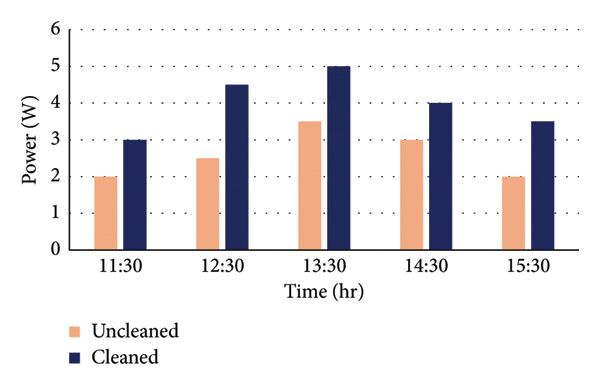
\includegraphics[width=0.92\linewidth]{grafico_soiling.jpg}
    \vspace{0.1cm}
    \end{minipage}
    \caption{Participação anual da solar fotovoltaica e da eólica na geração elétrica brasileira (esquerda, elaborado a partir de EPE, 2025 e 2026) e potência de painéis limpo e sujo ao longo do dia (direita, adaptado de Qi et al., 2025).}
    \label{fig:contexto_pesquisa}
    \vspace{-0.3cm}
\end{figure}

\section*{Materiais e Métodos}

O protótipo do sistema ASCM foi desenvolvido utilizando componentes comerciais de prateleira (COTS - \textit{Commercial Off-The-Shelf}) para manter o baixo custo de fabricação. O design estrutural e o mecanismo de movimentação linear foram modelados no software Autodesk Inventor, visando a prototipagem rápida através da fabricação por impressão 3D por deposição de material fundido (FDM). 

Para a confecção do protótipo físico de teste, utilizou-se filamento de PLA (Ácido Polilático) pela facilidade de impressão, embora materiais como PETG ou ABS possam ser aplicados em versões finais expostas a intempéries contínuas. A cremalheira linear (\textit{Gear-Rack}) é fixada ao longo das guias lineares do trilho de deslizamento e o pinhão (\textit{Gear} acoplado ao eixo do motor DC) engrena diretamente na cremalheira para guiar a translação suave do rodo de silicone através da peça de suporte do motor e do rodo (\textit{Wiper Support}), conforme o design CAD tridimensional em vista explodida (Figura \ref{fig:cad_design}).

\begin{figure}[htbp]
    \centering
    \begin{minipage}[b]{0.48\textwidth}
    \centering
    \IfFileExists{../images/vista_explodida.png}{%
        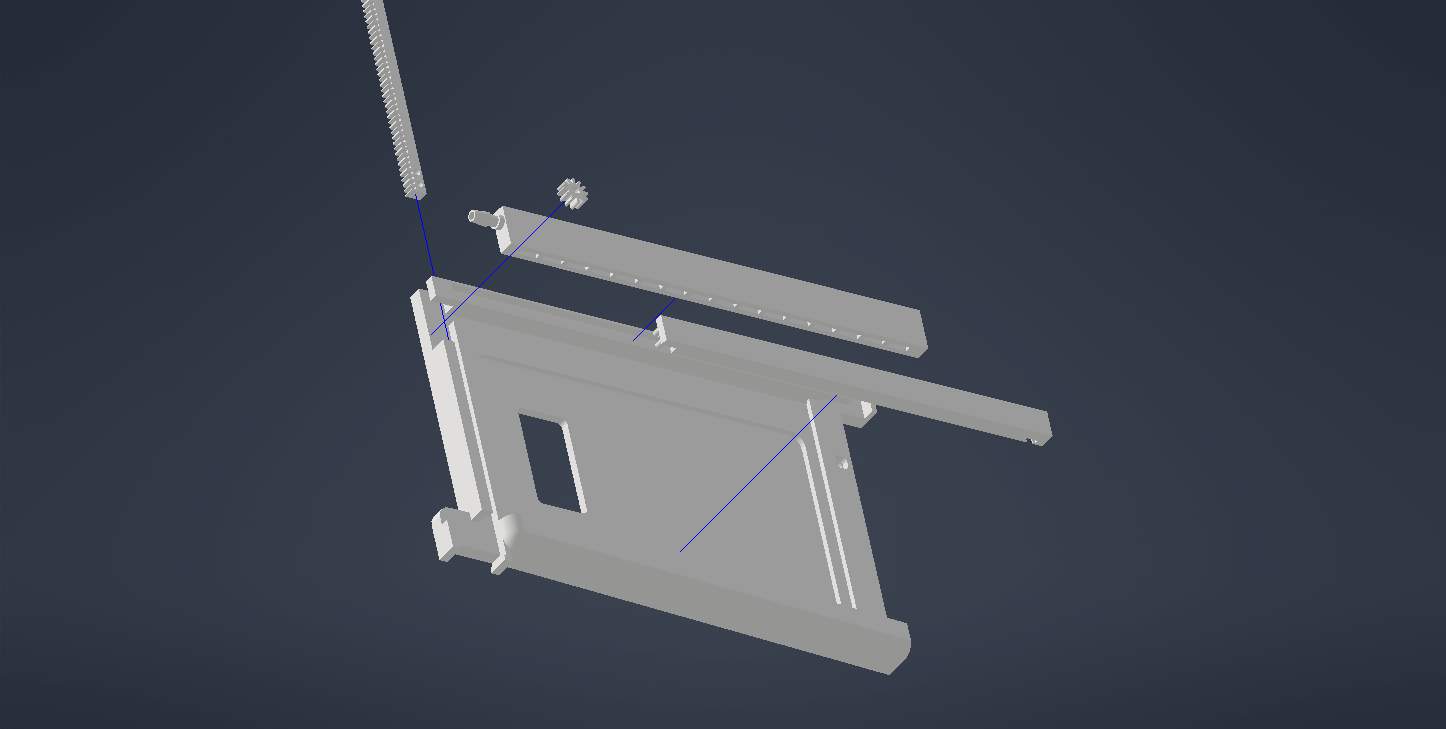
\includegraphics[width=\linewidth]{vista_explodida.png}%
    }{%
        \fbox{\parbox[c][4cm][c]{0.95\linewidth}{\centering\textit{Vista explodida da montagem (pendente)}}}%
    }
    \caption{Vista explodida da montagem do mecanismo de translação do ASCM: (1) Cremalheira (\textit{Gear-Rack}); (2) Pinhão (\textit{Gear}); (3) Suporte do Rodo (\textit{Wiper Support}); (4) Suporte de Aspersão (\textit{Sprinkler}); (5) Suporte dos Painéis (\textit{Panel Support}). Fonte: Elaborado pelos autores.}
    \label{fig:cad_design}
    \end{minipage}
    \hfill
    \begin{minipage}[b]{0.48\textwidth}
    \centering
    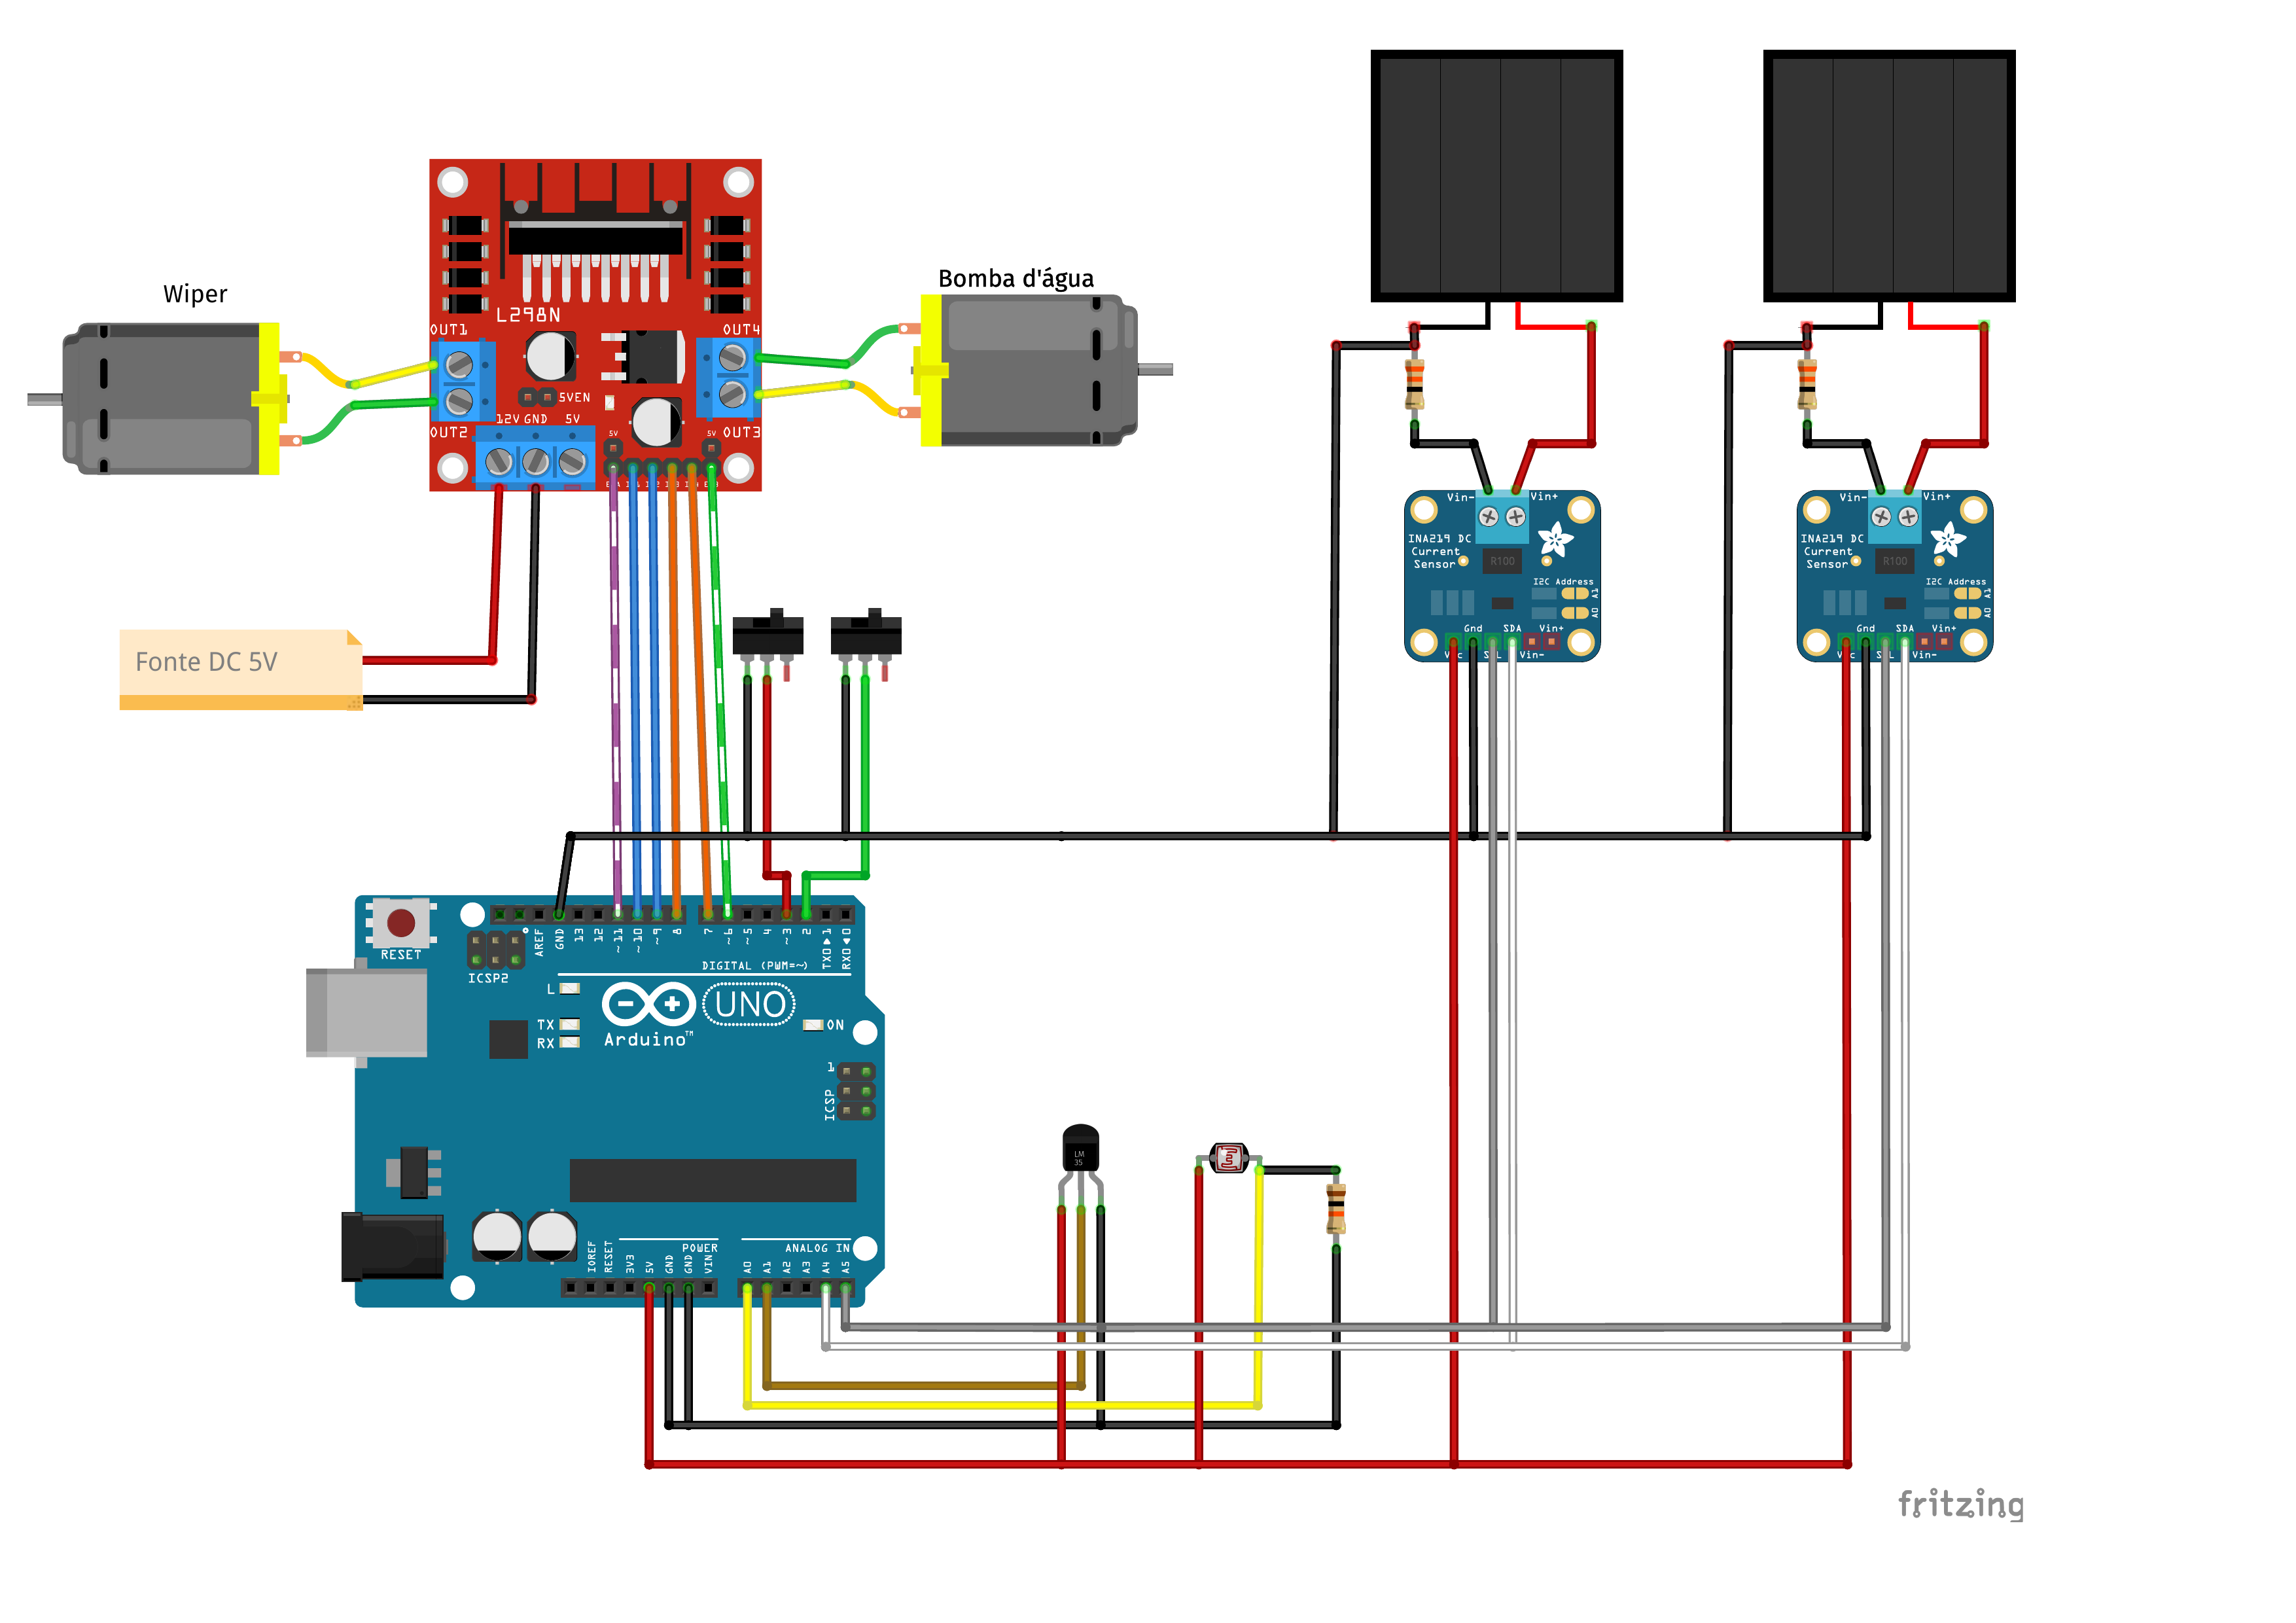
\includegraphics[width=0.85\linewidth]{diagrama_eletronica.png}
    \caption{Diagrama de conexões elétricas e esquemático de montagem física dos componentes eletrônicos do ASCM. Fonte: Elaborado pelos autores.}
    \label{fig:diagrama_eletronica}
    \end{minipage}
    \vspace{-0.3cm}
\end{figure}

O hardware eletrônico está centrado no microcontrolador Arduino Uno R3 (Figura \ref{fig:diagrama_eletronica}):
\begin{itemize}\setlength{\itemsep}{0pt}
    \item \textbf{Sensores INA219:} Dois módulos integrados via barramento $I^2C$ realizam a medição de corrente e tensão. O protótipo físico monitora o painel principal ($P_{main}$) e o compara ao painel de referência mantido limpo ($P_{ref}$), embora o sistema de software tenha sido idealizado sob a premissa de suportar a expansão de múltiplos nós em rede. Ambas as saídas são aplicadas sobre resistores de carga de 33 $\Omega$ e potência mínima de 1.5W.
    \item \textbf{Sensores Ambientais:} Um sensor analógico de luz (LDR) associado a um divisor de tensão de 10 k$\Omega$ estima a irradiância luminosa. A medição térmica da superfície é realizada por um termopar LM35 na face traseira do painel.
    \item \textbf{Atuadores:} O rodo mecânico é movido por um motor de corrente contínua (DC) acoplado a uma redução mecânica e acionado por um driver Ponte H L298N. Chaves fim de curso do tipo \textit{micro-switch} delimitam o movimento (\textit{limit\_home} e \textit{limit\_end}). Uma mini-bomba d'água submersível de 5V envia água aos bicos aspersores no topo do painel.
\end{itemize}


O controle do sistema adota a arquitetura \textbf{Telemetrix} \cite{telemetrix_doc}. O Arduino executa o sketch \textit{Telemetrix4Arduino}, operando como um servidor de I/O que se comunica via porta serial com um computador hospedeiro rodando um backend em Python (FastAPI) \cite{fastapi_doc} e um frontend em Streamlit \cite{streamlit_doc} (idealizados com suporte escalável para múltiplos nós). A estratégia de automação funciona em ciclo contínuo (Figura \ref{fig:fluxograma_controle}):
1. \textbf{Resfriamento Térmico:} A bomba de água é acionada em modo de fluxo alto por um período programado se a temperatura do painel ($T_{painel}$) superar o limiar térmico, isto é, se $T_{painel} > T_{amb} + \Delta T_{lim}$, onde $T_{amb}$ é a temperatura ambiente da API de clima e $\Delta T_{lim}$ é o diferencial limite (5$^\circ$C).
2. \textbf{Limpeza Automática:} A perda percentual por \textit{soiling} ($\Delta \eta$) é calculada em tempo real pela diferença de potência gerada entre o painel de referência mantido limpo ($P_{ref}$) e o painel principal monitorado ($P_{main}$):
\begin{equation} \label{eq:limpeza}
\Delta \eta = \left( \frac{P_{ref} - P_{main}}{P_{ref}} \right) \times 100\%
\end{equation}
Se $\Delta \eta > \eta_{lim}$ (limiar de sujeira tolerado, 10\%) e a API de clima indicar ausência de chuva, o ciclo é iniciado: a bomba molha a placa por 2 segundos, o wiper translada até o fim de curso progressivo, reverte o movimento até retornar ao ponto inicial e desliga o sistema.

O desenvolvimento colaborativo entre as frentes de eletrônica, mecânica e software foi gerenciado com Git e GitHub, permitindo a integração contínua do firmware com o backend e o frontend; o projeto está sob a licença de código aberto GPL v3.

\begin{figure}[htbp]
    \centering
    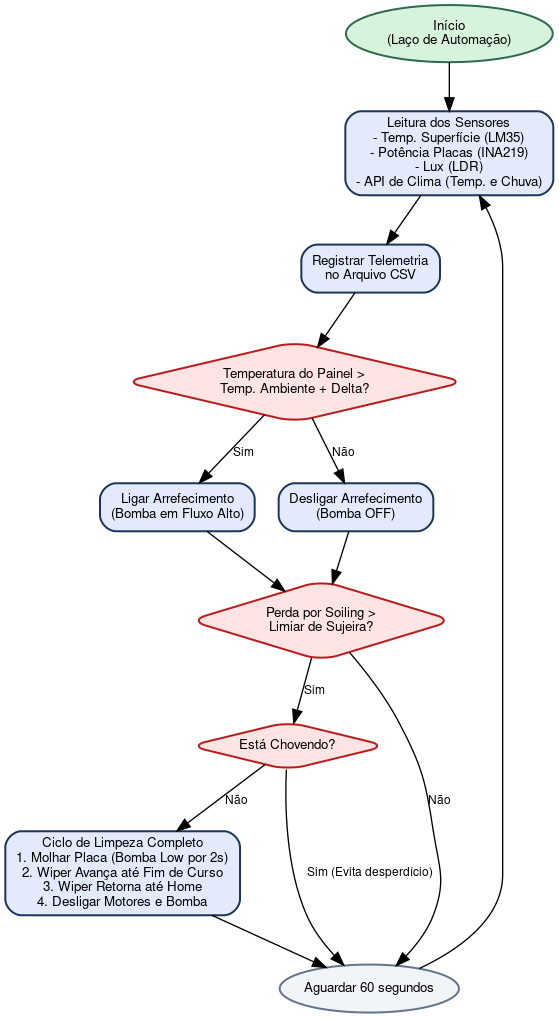
\includegraphics[width=0.85\linewidth]{fluxograma.png}
    \caption{Fluxograma do laço de controle de automação e de tomada de decisão do sistema ASCM. Fonte: Elaborado pelos autores.}
    \label{fig:fluxograma_controle}
    \vspace{-0.3cm}
\end{figure}

\section*{Resultados Preliminares e Discussão}

Durante as simulações e validações do software de controle, as rotinas de callback do Telemetrix integradas à biblioteca FastAPI demonstraram latência inferior a 15 ms para detecção das chaves fim de curso, garantindo uma parada de emergência segura para os motores de movimentação linear do rodo. Com a montagem do protótipo físico completo em andamento, será conduzido um ensaio experimental com o objetivo de comprovar a atenuação de eficiência e avaliar os ganhos trazidos pelo acionamento do sistema ASCM em escala de laboratório. Este ensaio de curto prazo com sujeira induzida serve como validação preliminar do laço de automação, sendo complementar a um ensaio de campo de longo prazo (30 dias, sujeira natural) planejado como etapa subsequente de validação em condições reais de operação. O procedimento do ensaio de curto prazo em ambiente controlado seguirá as seguintes etapas:
\begin{enumerate}\setlength{\itemsep}{0pt}
    \item O painel de referência limpo ($P_{ref}$) e o painel principal do protótipo ($P_{main}$) serão instalados sob um simulador solar de luz artificial (garantindo irradiância e temperatura estáveis).
    \item No instante inicial ($t=0$ min), ambos os painéis estarão limpos para calibração de base ($P_{main} \approx P_{ref}$).
    \item Será induzida poeira artificial de forma controlada e progressiva sobre o painel principal, monitorando-se a queda de tensão e corrente elétrica geradas, a fim de levantar a curva de soiling diferencial ($\Delta \eta$).
    \item Ao ultrapassar o limiar programado ($\eta_{lim} = 10\%$), o laço de controle do ASCM disparará o ciclo automático de aspersão com raspagem mecânica do rodo sobre o painel principal, medindo-se a recuperação instantânea de sua potência elétrica.
    \item Durante o ciclo, será registrada a corrente drenada da fonte de 5 V pela bomba e pelo motor, para o cálculo da energia consumida e do ganho energético líquido.
\end{enumerate}

Como os atuadores consomem energia, o benefício da limpeza é avaliado pelo ganho energético líquido:
\begin{equation} \label{eq:ganho_liquido}
E_{liq} = \int_{t_0}^{t_1} \left( P_{main}^{pós} - P_{main}^{pré} \right) dt - E_{ciclo}, \qquad E_{ciclo} = V_s \left( \bar{I}_b \, t_b + \bar{I}_m \, t_m \right)
\end{equation}
em que $[t_0, t_1]$ é o intervalo até o próximo ciclo, $V_s = 5$ V, e $\bar{I}_b$, $\bar{I}_m$, $t_b$ e $t_m$ são as correntes médias e os tempos de acionamento da bomba e do motor. No ciclo implementado, a bomba opera durante toda a limpeza (2 s de pré-umedecimento, avanço, 1 s de pausa e retorno) e cada curso do rodo é limitado por software a 30 s, logo $t_b \leq 63$ s e $t_m \leq 60$ s. Com valores nominais típicos (bomba $\approx$ 1 W; motorredutor $\approx$ 1,5 W), obtém-se o limite superior $E_{ciclo} \approx 153$ J ($\approx$ 0,04 Wh), compensado em cerca de 2,5 min pela recuperação de $\approx$ 1 W prevista na Tabela \ref{tab:ensaio_soiling}. Esses valores serão substituídos pelas correntes medidas, e o balanço será aplicado também ao arrefecimento e, em escala, ao consumo do Arduino e do computador hospedeiro.

A Tabela \ref{tab:ensaio_soiling} apresenta os dados estimados da atenuação de eficiência obtidos durante o ensaio controlado sob luz artificial constante, comprovando a perda de rendimento induzida e a posterior recuperação após a ativação do protótipo.

\begin{table}[htbp]
    \caption{Dados estimados para o ensaio de curto prazo com sujidade induzida sob luz artificial.}
    \vspace{.2cm}
    \centering
    \resizebox{\textwidth}{!}{%
    \begin{tabular}{cccccc}
    \hline
    \textbf{Tempo (min)} & \textbf{Irradiância Simulada} & \textbf{Potência Principal ($P_{main}$)} & \textbf{Potência Ref. Limpo ($P_{ref}$)} & \textbf{Perda por Soiling ($\Delta \eta$)} & \textbf{Status do Sistema} \\ \hline
    0 (Inicial) & 1000 W/m$^2$ & 9,50 W & 9,50 W & 0,0\% & Calibrado (Limpo) \\
    10 & 1000 W/m$^2$ & 9,21 W & 9,50 W & 3,1\% & Operacional \\
    20 & 1000 W/m$^2$ & 8,84 W & 9,50 W & 6,9\% & Operacional \\
    30 & 1000 W/m$^2$ & 8,45 W & 9,50 W & 11,1\% & Limpeza Ativada \\
    32 (Pós-Limpeza) & 1000 W/m$^2$ & 9,48 W & 9,50 W & 0,2\% & Eficiência Recuperada \\ \hline
    \end{tabular}%
    }
    \label{tab:ensaio_soiling}
\end{table}

Além disso, o termopar LM35 possibilitará a realização do ensaio térmico. Sob irradiância solar máxima no período do meio-dia (onde o painel atinge temperaturas superiores a 50$^\circ$C), o resfriamento evaporativo será acionado, mapeando a queda de temperatura vs o ganho de potência instantânea. Os resultados esperados preveem uma redução térmica estável de 5$^\circ$C a 10$^\circ$C na temperatura de operação das células, correspondendo a uma recuperação de potência de até 6,0\% no instante de resfriamento.

\section*{Conclusões}

O protótipo do ASCM projetado demonstrou-se viável sob o aspecto de desenvolvimento de software e integração de hardware de baixo custo, orçando um custo total de montagem inferior ao de soluções industriais. O uso do protocolo Telemetrix permitiu a criação de um laço de automação flexível e centralizado no computador hospedeiro via FastAPI e Streamlit. Os próximos passos consistem no término do acoplamento eletromecânico da rede de painéis e na execução prática do ensaio de curto prazo sob luz artificial para comprovação em escala física da remoção de sujidade induzida e testes térmicos. Espera-se com esses testes validar a eficácia prática da aspersão com raspagem mecânica na remoção de poeira consolidada (\textit{hard scale}).

%\section*{Contribuições dos Autores}
%
%L. E. contribuiu com: Concepção, Metodologia, Software, Investigação e Escrita – rascunho original. P. R. contribuiu com: Metodologia, Software, Recursos, Investigação, Visualização e Escrita – rascunho original. C. K. contribuiu com: Metodologia, Recursos, Investigação e Visualização. V. D. G. contribuiu com: Supervisão e Escrita – revisão e edição.

\section*{Agradecimentos}

Os autores agradecem ao Instituto Federal de Educação, Ciência e Tecnologia de São Paulo (IFSP) Câmpus São José dos Campos pelo apoio estrutural e pedagógico para o desenvolvimento deste projeto de iniciação tecnológica.

\bibliography{bibliografia.bib}

\end{document}
